\section{Static Design Structure Modeling}

\subsection{Diagram}
\begin{figure}[H]
   \centering
   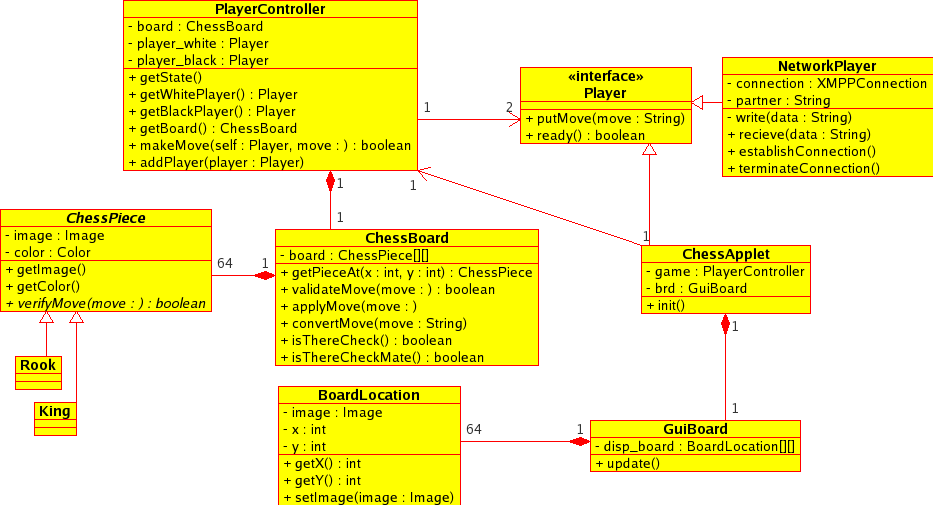
\includegraphics[scale=0.5]{cdiagram.png}
   \caption{Diagram illustrating the static interaction between components}
  \end{figure}
  %\FloatBarrier

\subsection{Descriptions}
\begin{description}
\item[D-10 PlayerController] - Handles the turn based model. Asks each player their move and posts each move to the other player (handles player to player communication)
\item[D-20 Player] - Provides a common interface between the controller and the local and networked player
\item[D-30 NetworkPlayer] - Handles sending move across the network and receiving moves sent across the network using XMPP as a backend
\item[D-40 ChessApplet] - Local player, applet that captures the moves and translates them for use
\item[D-50 ChessBoard] - Handles the state of the board, updating the board, and validates moves based on the current state of the board
\item[D-60 ChessPiece] - Handles how each piece moves, pieces inheriting this class implement a verifyMove method to verify each move (based on how a piece moves)
\item[D-70 BoardLocation] - Part of the gui that handles selecting a location (JButton)
\item[D-80 GuiBoard] - Handles drawing the board as a grid of BoardLocations


\end{description}
\begin{figure}[H]
   \centering
   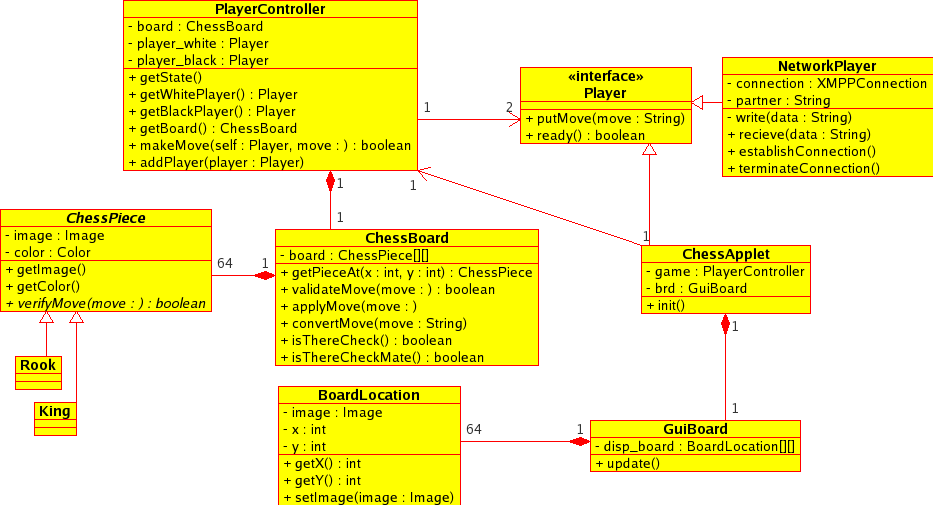
\includegraphics[angle=90,scale=0.85]{cdiagram.png}
   \caption{Diagram illustrating the static interaction between components}
  \end{figure}
  %\FloatBarrier
